% Options for packages loaded elsewhere
% Options for packages loaded elsewhere
\PassOptionsToPackage{unicode}{hyperref}
\PassOptionsToPackage{hyphens}{url}
\PassOptionsToPackage{dvipsnames,svgnames,x11names}{xcolor}
%
\documentclass[
  letterpaper,
  DIV=11,
  numbers=noendperiod]{scrartcl}
\usepackage{xcolor}
\usepackage{amsmath,amssymb}
\setcounter{secnumdepth}{-\maxdimen} % remove section numbering
\usepackage{iftex}
\ifPDFTeX
  \usepackage[T1]{fontenc}
  \usepackage[utf8]{inputenc}
  \usepackage{textcomp} % provide euro and other symbols
\else % if luatex or xetex
  \usepackage{unicode-math} % this also loads fontspec
  \defaultfontfeatures{Scale=MatchLowercase}
  \defaultfontfeatures[\rmfamily]{Ligatures=TeX,Scale=1}
\fi
\usepackage{lmodern}
\ifPDFTeX\else
  % xetex/luatex font selection
\fi
% Use upquote if available, for straight quotes in verbatim environments
\IfFileExists{upquote.sty}{\usepackage{upquote}}{}
\IfFileExists{microtype.sty}{% use microtype if available
  \usepackage[]{microtype}
  \UseMicrotypeSet[protrusion]{basicmath} % disable protrusion for tt fonts
}{}
\makeatletter
\@ifundefined{KOMAClassName}{% if non-KOMA class
  \IfFileExists{parskip.sty}{%
    \usepackage{parskip}
  }{% else
    \setlength{\parindent}{0pt}
    \setlength{\parskip}{6pt plus 2pt minus 1pt}}
}{% if KOMA class
  \KOMAoptions{parskip=half}}
\makeatother
% Make \paragraph and \subparagraph free-standing
\makeatletter
\ifx\paragraph\undefined\else
  \let\oldparagraph\paragraph
  \renewcommand{\paragraph}{
    \@ifstar
      \xxxParagraphStar
      \xxxParagraphNoStar
  }
  \newcommand{\xxxParagraphStar}[1]{\oldparagraph*{#1}\mbox{}}
  \newcommand{\xxxParagraphNoStar}[1]{\oldparagraph{#1}\mbox{}}
\fi
\ifx\subparagraph\undefined\else
  \let\oldsubparagraph\subparagraph
  \renewcommand{\subparagraph}{
    \@ifstar
      \xxxSubParagraphStar
      \xxxSubParagraphNoStar
  }
  \newcommand{\xxxSubParagraphStar}[1]{\oldsubparagraph*{#1}\mbox{}}
  \newcommand{\xxxSubParagraphNoStar}[1]{\oldsubparagraph{#1}\mbox{}}
\fi
\makeatother

\usepackage{color}
\usepackage{fancyvrb}
\newcommand{\VerbBar}{|}
\newcommand{\VERB}{\Verb[commandchars=\\\{\}]}
\DefineVerbatimEnvironment{Highlighting}{Verbatim}{commandchars=\\\{\}}
% Add ',fontsize=\small' for more characters per line
\usepackage{framed}
\definecolor{shadecolor}{RGB}{241,243,245}
\newenvironment{Shaded}{\begin{snugshade}}{\end{snugshade}}
\newcommand{\AlertTok}[1]{\textcolor[rgb]{0.68,0.00,0.00}{#1}}
\newcommand{\AnnotationTok}[1]{\textcolor[rgb]{0.37,0.37,0.37}{#1}}
\newcommand{\AttributeTok}[1]{\textcolor[rgb]{0.40,0.45,0.13}{#1}}
\newcommand{\BaseNTok}[1]{\textcolor[rgb]{0.68,0.00,0.00}{#1}}
\newcommand{\BuiltInTok}[1]{\textcolor[rgb]{0.00,0.23,0.31}{#1}}
\newcommand{\CharTok}[1]{\textcolor[rgb]{0.13,0.47,0.30}{#1}}
\newcommand{\CommentTok}[1]{\textcolor[rgb]{0.37,0.37,0.37}{#1}}
\newcommand{\CommentVarTok}[1]{\textcolor[rgb]{0.37,0.37,0.37}{\textit{#1}}}
\newcommand{\ConstantTok}[1]{\textcolor[rgb]{0.56,0.35,0.01}{#1}}
\newcommand{\ControlFlowTok}[1]{\textcolor[rgb]{0.00,0.23,0.31}{\textbf{#1}}}
\newcommand{\DataTypeTok}[1]{\textcolor[rgb]{0.68,0.00,0.00}{#1}}
\newcommand{\DecValTok}[1]{\textcolor[rgb]{0.68,0.00,0.00}{#1}}
\newcommand{\DocumentationTok}[1]{\textcolor[rgb]{0.37,0.37,0.37}{\textit{#1}}}
\newcommand{\ErrorTok}[1]{\textcolor[rgb]{0.68,0.00,0.00}{#1}}
\newcommand{\ExtensionTok}[1]{\textcolor[rgb]{0.00,0.23,0.31}{#1}}
\newcommand{\FloatTok}[1]{\textcolor[rgb]{0.68,0.00,0.00}{#1}}
\newcommand{\FunctionTok}[1]{\textcolor[rgb]{0.28,0.35,0.67}{#1}}
\newcommand{\ImportTok}[1]{\textcolor[rgb]{0.00,0.46,0.62}{#1}}
\newcommand{\InformationTok}[1]{\textcolor[rgb]{0.37,0.37,0.37}{#1}}
\newcommand{\KeywordTok}[1]{\textcolor[rgb]{0.00,0.23,0.31}{\textbf{#1}}}
\newcommand{\NormalTok}[1]{\textcolor[rgb]{0.00,0.23,0.31}{#1}}
\newcommand{\OperatorTok}[1]{\textcolor[rgb]{0.37,0.37,0.37}{#1}}
\newcommand{\OtherTok}[1]{\textcolor[rgb]{0.00,0.23,0.31}{#1}}
\newcommand{\PreprocessorTok}[1]{\textcolor[rgb]{0.68,0.00,0.00}{#1}}
\newcommand{\RegionMarkerTok}[1]{\textcolor[rgb]{0.00,0.23,0.31}{#1}}
\newcommand{\SpecialCharTok}[1]{\textcolor[rgb]{0.37,0.37,0.37}{#1}}
\newcommand{\SpecialStringTok}[1]{\textcolor[rgb]{0.13,0.47,0.30}{#1}}
\newcommand{\StringTok}[1]{\textcolor[rgb]{0.13,0.47,0.30}{#1}}
\newcommand{\VariableTok}[1]{\textcolor[rgb]{0.07,0.07,0.07}{#1}}
\newcommand{\VerbatimStringTok}[1]{\textcolor[rgb]{0.13,0.47,0.30}{#1}}
\newcommand{\WarningTok}[1]{\textcolor[rgb]{0.37,0.37,0.37}{\textit{#1}}}

\usepackage{longtable,booktabs,array}
\newcounter{none} % for unnumbered tables
\usepackage{calc} % for calculating minipage widths
% Correct order of tables after \paragraph or \subparagraph
\usepackage{etoolbox}
\makeatletter
\patchcmd\longtable{\par}{\if@noskipsec\mbox{}\fi\par}{}{}
\makeatother
% Allow footnotes in longtable head/foot
\IfFileExists{footnotehyper.sty}{\usepackage{footnotehyper}}{\usepackage{footnote}}
\makesavenoteenv{longtable}
\usepackage{graphicx}
\makeatletter
\newsavebox\pandoc@box
\newcommand*\pandocbounded[1]{% scales image to fit in text height/width
  \sbox\pandoc@box{#1}%
  \Gscale@div\@tempa{\textheight}{\dimexpr\ht\pandoc@box+\dp\pandoc@box\relax}%
  \Gscale@div\@tempb{\linewidth}{\wd\pandoc@box}%
  \ifdim\@tempb\p@<\@tempa\p@\let\@tempa\@tempb\fi% select the smaller of both
  \ifdim\@tempa\p@<\p@\scalebox{\@tempa}{\usebox\pandoc@box}%
  \else\usebox{\pandoc@box}%
  \fi%
}
% Set default figure placement to htbp
\def\fps@figure{htbp}
\makeatother





\setlength{\emergencystretch}{3em} % prevent overfull lines

\providecommand{\tightlist}{%
  \setlength{\itemsep}{0pt}\setlength{\parskip}{0pt}}



 


\KOMAoption{captions}{tableheading}
\makeatletter
\@ifpackageloaded{caption}{}{\usepackage{caption}}
\AtBeginDocument{%
\ifdefined\contentsname
  \renewcommand*\contentsname{Table of contents}
\else
  \newcommand\contentsname{Table of contents}
\fi
\ifdefined\listfigurename
  \renewcommand*\listfigurename{List of Figures}
\else
  \newcommand\listfigurename{List of Figures}
\fi
\ifdefined\listtablename
  \renewcommand*\listtablename{List of Tables}
\else
  \newcommand\listtablename{List of Tables}
\fi
\ifdefined\figurename
  \renewcommand*\figurename{Figure}
\else
  \newcommand\figurename{Figure}
\fi
\ifdefined\tablename
  \renewcommand*\tablename{Table}
\else
  \newcommand\tablename{Table}
\fi
}
\@ifpackageloaded{float}{}{\usepackage{float}}
\floatstyle{ruled}
\@ifundefined{c@chapter}{\newfloat{codelisting}{h}{lop}}{\newfloat{codelisting}{h}{lop}[chapter]}
\floatname{codelisting}{Listing}
\newcommand*\listoflistings{\listof{codelisting}{List of Listings}}
\makeatother
\makeatletter
\makeatother
\makeatletter
\@ifpackageloaded{caption}{}{\usepackage{caption}}
\@ifpackageloaded{subcaption}{}{\usepackage{subcaption}}
\makeatother
\usepackage{bookmark}
\IfFileExists{xurl.sty}{\usepackage{xurl}}{} % add URL line breaks if available
\urlstyle{same}
% fallback for those not using the hyperref driver hyperxmp:
\makeatletter
\@ifundefined{xmpquote}{\newcommand{\xmpquote}[1]{#1}}{}
\makeatother
\hypersetup{
  pdftitle={An Introduction to the Usefulness of Bayesian Inference},
  pdfauthor={Dallin Anderson},
  colorlinks=true,
  linkcolor={blue},
  filecolor={Maroon},
  citecolor={Blue},
  urlcolor={Blue},
  pdfcreator={LaTeX via pandoc}}


\title{An Introduction to the Usefulness of Bayesian Inference}
\author{Dallin Anderson}
\date{}
\begin{document}
\maketitle


\section{Beginning}\label{beginning}

When a Data Scientist exits the realm of collegiate education, they come
prepared with the skills to answer questions about big data using
statistics and the methods they have developed in their languages.
However, the world of data is ever expanding and always changing.
Sometimes the data you need does not exist yet and an expensive
experiment is required to gather it. Sometimes it does exist but not
much has been recorded for some various reason. How then is our newly
endowed graduate expected to handle solving a problem when the data
isn't as big as they expected?

This problem is often found in the nooks of small businesses, eager to
hire our college graduate because the bigger the fish the stronger the
bait needed to hook them. And as we have said, they are small tugboats
in a world of oceanliners. They can't afford to get the big data, nor
can they afford the PhD statisticians. So they look towards our graduate
for hope. What hope is there?

Well, when data is available by the bushel and collects like rain from a
Midwest storm, standard frequentist methods will suffice. They assume
LINE assumptions are met because in the vast buckets and buckets of data
available to them, small outliers aren't enough to shift the expected
value to a great degree. But because data might not be as available as
one would be lead to believe, the skilled statistician will keep a few
bayesian methods in their back pocket, to whip out as a secret magic
trick when their usual routine falls flat.

\section{Bayes and His Theorem}\label{bayes-and-his-theorem}

Bayesian statistics gets its name from the man Thomas Bayes, who flipped
the script in regards to what statistics was. Rather than treating
probability as a fixed value of frequency, he believed probability to be
the representation of belief and can update when new information is
received. (History)

The main draw though isn't how data is perceived. Nor is it that
bayesian statistics is easier than the popular frequentist methods,
though some may argue that in many cases that is true. Rather Bayes
provided a path for statistics that is probabilistically consistent.
Meaning that as the data gets harder, more complex, less normal, the
framework of bayesian statistics stays the same.

Let's do a quick overview of the math before getting into actually
putting a model into practice. Commonly in Statistics we know that

\(\( P(A \mid B) = \frac{P(A \cap B)}{P(B)} \)\)

Bayes looked at this relationship and realized that by multiplying the
probability in the denominator to the other side, the math could be
manipulated into the following, known now as the Bayesian Theorem.

\(\( P(A \mid B) = \frac{P(B \mid A)\,P(A)}{P(B)} \)\)

In applying the bayesian method, we redefine what each of these
probabilities mean.

\(\( P(parameters \mid data) = \frac{P(data \mid parameters)\,P(parameters)}{P(data)} \)\)

With more study, Bayes realized the following identity about the
relationship between data and our parameters. The posterior we are
looking for, being the parameters given data, is proportional to a
function of the likelihood and priors, the likelihood being data given
parameters and our prior being the probability of each parameter.

\(\( p(\theta \mid y) \propto p(y \mid \theta)\,p(\theta) \)\)

This is the foundational knowledge of bayesian statistics. That if we
can determine priors: what we think should happen and a small sample
from the population; as well as the likelihood of our data: the sampling
density or better yet the function our data might take; we can produce a
posterior that represents what our parameters are like given our data.

\section{What's the Point}\label{whats-the-point}

The issue was, trying to create a posterior distribution by hand is
incredibly annoying. For a long time people dismissed bayesian ideas
because they just weren't practical. The Monte Carlo simulation methods
changed everything. Now there was a way to create distributions given
general inputs and simulate large amounts of data reliably. With that
tool, the bayesian ideal became possible. Given a prior and a
likelihood, a person could use data to simulate draws from a large
population with only a small amount of samples. As long as the priors
were well informed, the data was sound, though less data meant priors
had greater influence.

What does that mean exactly? Well, we can simulate what we think the
population might look like, given our data no matter how small. Want to
know what your company might be worth? Now you can create that
population without ever entering the stock market! Want to know if a
drug is effective? Now you can for a fraction of the cost! Bayesian
methods empower those with less access to data or the finances to
collect it to do more as long as the research into the priors is sound.
Best of all, because the data is simulated using methods grounded in
mathematics, hypothesis tests and other statistics are no longer vague
values you have to estimate. No, you can know the exact probability,
with absolute confidence. Parameters themselves are not fixed and
unknown. They are a function of their probability, which you know
because of the simulated population.

Simply put, the metrics that frequentists warn for a statistician to be
wary of, making sure your diagnostics are correct, can be confidently
stated by the bayesian and backed up by hard evidence of what priors
they chose and why. Statistics moves from the realm of interpretable to
empirical.

\section{Bayes in Action}\label{bayes-in-action}

Let's do an example. In R, we use the Nimble or STAN code to simulate
MCMC draws from a posterior distribution, but with the object oriented
language of Python at our fingertips, we can do the same but faster. It
should be noted though that STAN code is rather versatile across many
environments, including Python, so an understanding of STAN may be more
useful to the aspiring bayesian thinker. The following code uses the
\emph{PyMC} and \emph{Arviz} packages to accomplish the task.

\emph{PyMC} is a package that functions similar to Nimble code, so I
have utilized it as I am more familiar with Nimble's way of doing
things. Another popular package is \emph{NumPyro} which has a harder
learning curve but is more data efficient. \emph{Arviz} is a diagnostic
package that allows us to check the convergence and relevant statistics
to determine if the model we produced is able to be used.

For our demonstration we will be using a 2x33 dataframe that contains
two treatments in one column and a response in the other. Imagine these
the metrics of a two types of social media posts and the number of views
as the response, but you only have a week until launch so you could only
collect 33 hours of data to work with. Or maybe it's two drugs affecting
blood pressure. Choose any number of examples you want. For our
purposes, we'll stick with the social media example. Either way, a
frequentist would say the sample size is barely big enough to meet the
Central Limit Theorem but with so few samples the power of the study is
rather small. However, a bayesian would be right at home.

One last note, bayesian statistics uses a lot of computational power in
order to simulate the population. \emph{PyMC} tends to use PyTensor and
BLAS/LAPACK compilers that may not be loaded on your computer. We can
bypass this by importing the \emph{nutpie} sampler which does not rely
on these powerful but draining tools.

\begin{Shaded}
\begin{Highlighting}[]
\ImportTok{import}\NormalTok{ pandas }\ImportTok{as}\NormalTok{ pd}
\ImportTok{import}\NormalTok{ pymc }\ImportTok{as}\NormalTok{ pm}
\ImportTok{import}\NormalTok{ arviz }\ImportTok{as}\NormalTok{ az}
\ImportTok{import}\NormalTok{ numpy }\ImportTok{as}\NormalTok{ np}
\ImportTok{import}\NormalTok{ nutpie}


\NormalTok{exc }\OperatorTok{=}\NormalTok{ pd.read\_csv(}
    \StringTok{"Data/exercises3.dat"}\NormalTok{,}
\NormalTok{    sep}\OperatorTok{=}\VerbatimStringTok{r"}\DecValTok{\textbackslash{}s}\OperatorTok{+}\VerbatimStringTok{"}\NormalTok{,}
\NormalTok{    header}\OperatorTok{=}\VariableTok{None}\NormalTok{,}
\NormalTok{    names}\OperatorTok{=}\NormalTok{[}\StringTok{"V1"}\NormalTok{, }\StringTok{"V2"}\NormalTok{]}
\NormalTok{)}

\NormalTok{tmt }\OperatorTok{=}\NormalTok{ exc[}\StringTok{\textquotesingle{}V1\textquotesingle{}}\NormalTok{].values          }\CommentTok{\# treatments (1 or 2)}
\NormalTok{y }\OperatorTok{=}\NormalTok{ exc[}\StringTok{\textquotesingle{}V2\textquotesingle{}}\NormalTok{].values            }\CommentTok{\# responses}
\NormalTok{n\_groups }\OperatorTok{=} \BuiltInTok{len}\NormalTok{(np.unique(tmt))}
\NormalTok{tmt\_idx }\OperatorTok{=}\NormalTok{ tmt }\OperatorTok{{-}} \DecValTok{1}   \CommentTok{\# convert \{1,2\} → \{0,1\} to work with PyMC}
\end{Highlighting}
\end{Shaded}

\begin{verbatim}
g++ not available, if using conda: `conda install gxx`
\end{verbatim}

Here you can view a bit of the data

\begin{Shaded}
\begin{Highlighting}[]
\NormalTok{exc.head()}
\end{Highlighting}
\end{Shaded}

{\def\LTcaptype{none} % do not increment counter
\begin{longtable}[]{@{}lll@{}}
\toprule\noalign{}
& V1 & V2 \\
\midrule\noalign{}
\endhead
\bottomrule\noalign{}
\endlastfoot
0 & 1 & 121 \\
1 & 1 & 94 \\
2 & 1 & 119 \\
3 & 1 & 122 \\
4 & 1 & 142 \\
\end{longtable}
}

\begin{Shaded}
\begin{Highlighting}[]
\NormalTok{exc.tail()}
\end{Highlighting}
\end{Shaded}

{\def\LTcaptype{none} % do not increment counter
\begin{longtable}[]{@{}lll@{}}
\toprule\noalign{}
& V1 & V2 \\
\midrule\noalign{}
\endhead
\bottomrule\noalign{}
\endlastfoot
28 & 2 & 126 \\
29 & 2 & 127 \\
30 & 2 & 111 \\
31 & 2 & 112 \\
32 & 2 & 121 \\
\end{longtable}
}

With our data loaded, now we need to build our model. Remember, our goal
is to create a posterior distribution from which we can draw from,
simulating our population. To do that, we need to establish our priors,
or rather what we think the data should look like. Keeping with our
social media example, say we did some research and found that newly
created channels on our given platform, when marketed for the first
time, get around 120 views. As our sample is derived from someone's
natural response, we want a normal distribution. Our posterior, for
reasons too complicated to explain in a single post, will then be a
Normal distribution as well. For safety, we'll be cautious and set that
expected prior for our mean, or \textbf{mu}, at a standard deviation of
20 views. Our prior for the standard deviation of our expected is
unbiased, because we don't know the variance of how people interact on
our given site. Thus we'll keep it at a standard gamma prior.

Then we define how we want to sample from the distribution. The general
idea is to take as many draws as possible, but we want to balance the
effectiveness of our model with the computational power we are using. I
tried being ambitious and setting the model to have 16,000 draws during
testing, but it took over 30 minutes to run which isn't effective on my
lone computer. For this demo, we've set it to 2,000 draws per chain. We
perform multiple chains because of the Fisher design principle of
repetition. We would only do one chain, but who's to say that our model
isn't flawed? Multiple chains help to establish a model's effectiveness
and let us see if our priors are making our mean too unstable.

Next we tune the model. Tuning removes the first 1000 draws as the MCMC
needs time to reach convergence and we don't want that period of time
where we are warming up our engines to be caught as actual time in the
race. So in actuality our model will only end up with 1,000 draws by the
end. In R we would also thin to remove dependence on the draws. MCMC is
effective but sometimes the lag time between each draw might be high,
meaning that the result of sample 1456 is closely related to sample
1457. We thin to remove that autocorrelation. However, PyMC is far
better at producing less autocorrelated values than Nimble is so we
don't include it here.

\begin{Shaded}
\begin{Highlighting}[]
\ControlFlowTok{with}\NormalTok{ pm.Model() }\ImportTok{as}\NormalTok{ exc\_model:}
    
    \CommentTok{\# Priors for each treatment group}
\NormalTok{    mu }\OperatorTok{=}\NormalTok{ pm.Normal(}\StringTok{"mu"}\NormalTok{, mu}\OperatorTok{=}\DecValTok{120}\NormalTok{, sigma}\OperatorTok{=}\DecValTok{20}\NormalTok{, shape}\OperatorTok{=}\NormalTok{n\_groups)}
\NormalTok{    s }\OperatorTok{=}\NormalTok{ pm.Gamma(}\StringTok{"s"}\NormalTok{, alpha}\OperatorTok{=}\FloatTok{1.1}\NormalTok{, beta}\OperatorTok{=}\FloatTok{0.1}\NormalTok{, shape}\OperatorTok{=}\NormalTok{n\_groups)}
    
    \CommentTok{\# Likelihood}
\NormalTok{    y\_obs }\OperatorTok{=}\NormalTok{ pm.Normal(}\StringTok{"y\_obs"}\NormalTok{, mu}\OperatorTok{=}\NormalTok{mu[tmt\_idx], sigma}\OperatorTok{=}\NormalTok{s[tmt\_idx], observed}\OperatorTok{=}\NormalTok{y)}
    
    \CommentTok{\# Sampling}
\NormalTok{    trace }\OperatorTok{=}\NormalTok{ pm.sample(}
\NormalTok{        draws}\OperatorTok{=}\DecValTok{2000}\NormalTok{,}
\NormalTok{        tune}\OperatorTok{=}\DecValTok{1000}\NormalTok{,}
\NormalTok{        chains}\OperatorTok{=}\DecValTok{4}\NormalTok{,}
\NormalTok{        target\_accept}\OperatorTok{=}\FloatTok{0.9}\NormalTok{,}
\NormalTok{        nuts\_sampler}\OperatorTok{=}\StringTok{"nutpie"}\NormalTok{,}
\NormalTok{    )}
\end{Highlighting}
\end{Shaded}

\begin{verbatim}
NUTS[nutpie]: [mu, s]
\end{verbatim}

\begin{verbatim}
Output()
\end{verbatim}

\begin{verbatim}
\end{verbatim}

The diagnostics below are important in checking that our posterior
distribution converged, or rather that the distribution functions as
expected. If it was constantly increasing infinitely, we would know that
our probability could not converge to 1 and thus our analysis would be
void. A good trace plot should be centered on the plot as much as
possible and stay at a steady line with no drastic curves upward or
downward

\begin{Shaded}
\begin{Highlighting}[]
\CommentTok{\# Trace plots}
\NormalTok{az.plot\_trace(trace)}
\end{Highlighting}
\end{Shaded}

\pandocbounded{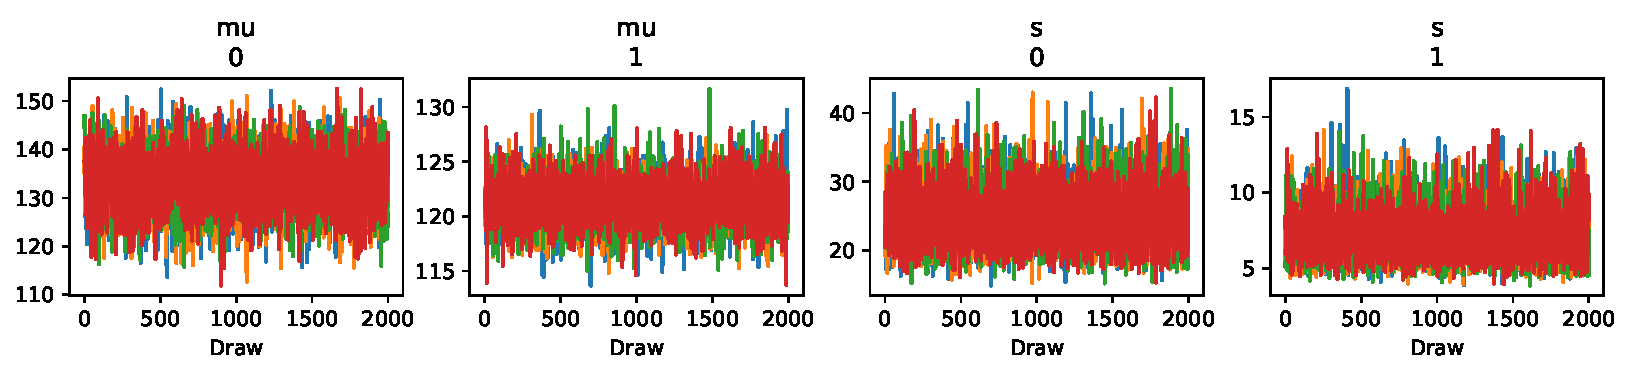
\includegraphics[keepaspectratio]{Tutorial_files/figure-pdf/cell-6-output-1.pdf}}

Autocorrelation looks at how correlated each produced is to each other
by a metric called lag. A lag of 2 implies the correlation between one
value and the value 2 steps after it. We want a very low autocorrelation
since a high metric would imply one sample depends on another,
invalidating the data.

\begin{Shaded}
\begin{Highlighting}[]
\CommentTok{\# Autocorrelation}
\NormalTok{az.plot\_autocorr(trace)}
\end{Highlighting}
\end{Shaded}

\pandocbounded{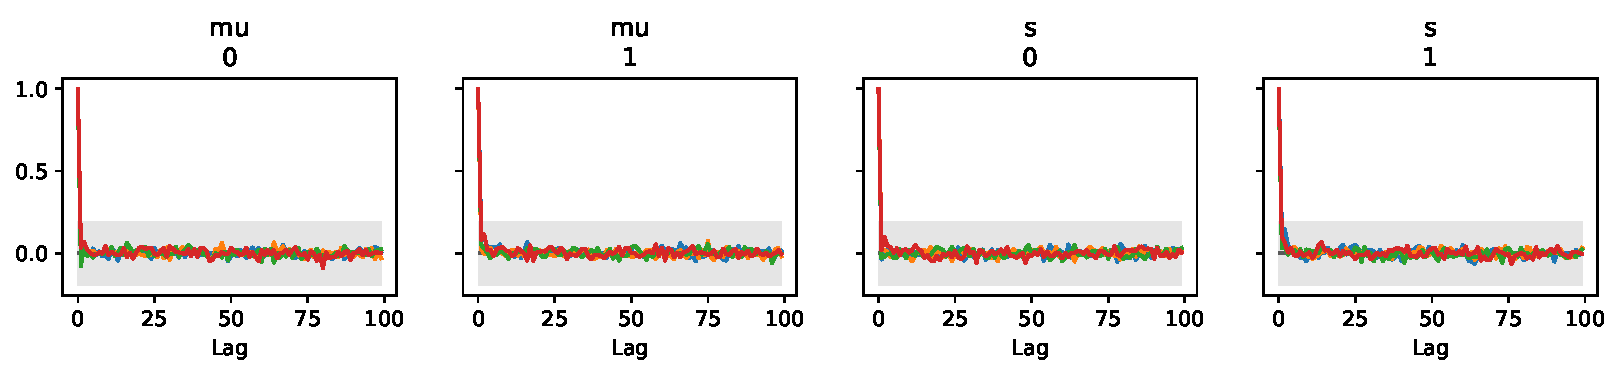
\includegraphics[keepaspectratio]{Tutorial_files/figure-pdf/cell-7-output-1.pdf}}

Finally we can look at the values produced by our posterior
distribution, including the two means and two standard deviations that
were generated based on our priors and likelihood. ess\_bulk tells us
the effective sample size, or how many of the generated samples from the
chains are actually usable. A value of at least 6000 is preferred, which
we barely met for our 2nd mu. Rhat, or the Gelman--Rubin statistic,
checks that each of the chains converged to the same posterior
distribution. We want the values as close to 1 as possible, with 1.05 or
higher being bad. The other metrics refer to the credible intervals for
the mu/sd (the eti 89\% lower and upper bounds), how well sampled the
distribution tails are (ess\_tail), and the uncertainty of the sampling
process itself, the Monte Carlo Standard Error.

\begin{Shaded}
\begin{Highlighting}[]
\CommentTok{\# Summary table (Rhat, ESS, quantiles)}
\NormalTok{az.summary(trace)}
\end{Highlighting}
\end{Shaded}

{\def\LTcaptype{none} % do not increment counter
\begin{longtable}[]{@{}llllllllll@{}}
\toprule\noalign{}
& mean & sd & eti89\_lb & eti89\_ub & ess\_bulk & ess\_tail & r\_hat &
mcse\_mean & mcse\_sd \\
\midrule\noalign{}
\endhead
\bottomrule\noalign{}
\endlastfoot
mu{[}0{]} & 133.5 & 5.5 & 120 & 140 & 7589 & 5244 & 1.00 & 0.064 &
0.069 \\
mu{[}1{]} & 121.42 & 1.97 & 120 & 120 & 5925 & 4749 & 1.00 & 0.026 &
0.029 \\
s{[}0{]} & 24.63 & 3.91 & 19 & 32 & 8067 & 5626 & 1.00 & 0.045 &
0.049 \\
s{[}1{]} & 7.15 & 1.52 & 5.2 & 9.8 & 6593 & 4981 & 1.00 & 0.02 &
0.022 \\
\end{longtable}
}

Now, what if we wanted to perform a regression model? In a frequentist
world, we need a new formula with new assumption and yada yada yada.
Bayesian statistics doesn't need that. Simply define your \textbf{y} and
\textbf{mu} as you would in a regression model, and bam! You're good to
go! Validation is the same and the resulting statistics are tangible.
The process changes slightly to account for the different analysis but
the framework is the same. Such is the power of bayesian statistics.

\begin{Shaded}
\begin{Highlighting}[]
\ControlFlowTok{with}\NormalTok{ pm.Model() }\ImportTok{as}\NormalTok{ exc\_model\_regression:}

    \CommentTok{\# Priors for regression coefficients}
\NormalTok{    alpha }\OperatorTok{=}\NormalTok{ pm.Normal(}\StringTok{"alpha"}\NormalTok{, mu}\OperatorTok{=}\DecValTok{120}\NormalTok{, sigma}\OperatorTok{=}\DecValTok{20}\NormalTok{)        }\CommentTok{\# intercept}
\NormalTok{    beta  }\OperatorTok{=}\NormalTok{ pm.Normal(}\StringTok{"beta"}\NormalTok{, mu}\OperatorTok{=}\DecValTok{0}\NormalTok{,   sigma}\OperatorTok{=}\DecValTok{10}\NormalTok{)         }\CommentTok{\# slope for treatment effect}

    \CommentTok{\# Prior for residual standard deviation}
\NormalTok{    sigma }\OperatorTok{=}\NormalTok{ pm.Gamma(}\StringTok{"sigma"}\NormalTok{, alpha}\OperatorTok{=}\FloatTok{1.1}\NormalTok{, beta}\OperatorTok{=}\FloatTok{0.1}\NormalTok{)}

    \CommentTok{\# Expected value of each observation}
\NormalTok{    mu }\OperatorTok{=}\NormalTok{ alpha }\OperatorTok{+}\NormalTok{ beta }\OperatorTok{*}\NormalTok{ tmt   }\CommentTok{\# regression mean}

    \CommentTok{\# Likelihood}
\NormalTok{    y\_obs }\OperatorTok{=}\NormalTok{ pm.Normal(}\StringTok{"y\_obs"}\NormalTok{, mu}\OperatorTok{=}\NormalTok{mu, sigma}\OperatorTok{=}\NormalTok{sigma, observed}\OperatorTok{=}\NormalTok{y)}

    \CommentTok{\# Sampling}
\NormalTok{    trace }\OperatorTok{=}\NormalTok{ pm.sample(}
\NormalTok{        draws}\OperatorTok{=}\DecValTok{2000}\NormalTok{,}
\NormalTok{        tune}\OperatorTok{=}\DecValTok{1000}\NormalTok{,}
\NormalTok{        chains}\OperatorTok{=}\DecValTok{4}\NormalTok{,}
\NormalTok{        target\_accept}\OperatorTok{=}\FloatTok{0.9}\NormalTok{,}
\NormalTok{        nuts\_sampler}\OperatorTok{=}\StringTok{"nutpie"}\NormalTok{,}
\NormalTok{    )}
\end{Highlighting}
\end{Shaded}

Because our distribution passed the validation checks, we can pull the
samples and perform a hypothesis check easily. In this case, the exact
probability that mu2 is greater than mu1.

\begin{Shaded}
\begin{Highlighting}[]
\NormalTok{mu\_samples }\OperatorTok{=}\NormalTok{ trace.posterior[}\StringTok{"mu"}\NormalTok{].stack(draws}\OperatorTok{=}\NormalTok{(}\StringTok{"chain"}\NormalTok{, }\StringTok{"draw"}\NormalTok{)).values}
\NormalTok{prob\_mu2\_gt\_mu1 }\OperatorTok{=}\NormalTok{ np.mean(mu\_samples[:,}\DecValTok{1}\NormalTok{] }\OperatorTok{\textgreater{}}\NormalTok{ mu\_samples[:,}\DecValTok{0}\NormalTok{])}
\BuiltInTok{print}\NormalTok{(prob\_mu2\_gt\_mu1)}
\end{Highlighting}
\end{Shaded}

\begin{verbatim}
0.5
\end{verbatim}

If the person we are giving this info to questions whether the data is
reliable, we don't need to figure out how to explain complex statistics
metrics into common sense. We can simply discuss what we knew, how we
factored that into making our distribution, and that the model passed
validation checks. And since our model produced a posterior distribution
with draws, we can simulate events using the found mu2 and sd2, called
the posterior predictive distribution. In this case, we predict about
126 views per hour for our social media method 2.

\begin{Shaded}
\begin{Highlighting}[]
\NormalTok{mu2 }\OperatorTok{=}\NormalTok{ mu\_samples[:,}\DecValTok{1}\NormalTok{]}
\NormalTok{s2  }\OperatorTok{=}\NormalTok{ trace.posterior[}\StringTok{"s"}\NormalTok{].stack(draws}\OperatorTok{=}\NormalTok{(}\StringTok{"chain"}\NormalTok{,}\StringTok{"draw"}\NormalTok{)).values[:,}\DecValTok{1}\NormalTok{]}

\NormalTok{postpred }\OperatorTok{=}\NormalTok{ np.random.normal(mu2, s2)}
\BuiltInTok{print}\NormalTok{(postpred.mean())}
\end{Highlighting}
\end{Shaded}

\begin{verbatim}
130.836084770896
\end{verbatim}

\section{Practical Applications}\label{practical-applications}

This is the power of bayesian statistics. Because we can trace back and
explain every part of our model mathematically, the results we produce
are empirical and decisive, with fixed bounds. There is no such thing as
confidence, because we can produce credible results. It's a huge game
changer. If we want to introduce a new technology to the market,
bayesian statistics lets us predict its success, to a degree, without
ever creating a survey. It's an awesome tool for small businesses and
for large ones that want to save money. More so, it's a new way of
thinking about statistics, which lends itself to even greater
applications.

One final example of the potential of bayesian statistics is its use in
Large Language Models, the technology that powers AI agents. A
bottleneck in building these is the training process which requires
massive amounts of data to be fed into the model and analyzed.
\href{https://doi.org/10.1038/s41467-025-67998-6}{Bayesian teaching
enables probabilistic reasoning in large language models} is a paper
published at the start of 2026 and argues that training LLMs on the
basics of bayesian inference improves their reasoning abilities, meaning
they learn faster and more reliably. Those going into data science would
be remiss not having the knowledge to improve their models, and at a
cheaper cost because of bayesian statistics.

\section{Learn More}\label{learn-more}

Though we have covered the bare basics of bayesian methods in our
exploration, the opportunities to study this topic are only growing
since their inception. Brigham Young University has been leading the
charge, with several professors having a background in the bayesian
methods. As of writing, the STAT 251 class will introduce the
foundations needed to understand the methodology. Then a student can
choose between STAT 466 which focuses on developing an understanding of
bayesian theory through mathematics or STAT 451 which dives into the
code to implement bayesian methods. The python code demonstrated today
draws from the syntax taught in the latter.

Do not fret though! If academic curriculum lay beyond your reach,
Gilbert W. Fellingham and Scott A. Baldwin have answered your unsung
lamentations with their book \emph{An Introduction to Applied Bayesian
Methods}. Releasing in November of 2026, this text covers what would be
taught in the STAT 451 course and provides the R-code to immediately
apply the methods they preach. I was given early access to the text and
while it is less complex than your standard tome it boasts
industry-applicable tools to get you on your way. Much of what was
discussed in this article pulls from that book. Highly recommend picking
up a copy.

Bayesian statistics may not be as popular as our tried and true
frequentist friends but the hope is after reading you may be convinced,
if only ever so slightly, to prepare amongst your tricks a bayesian
method or two. For though the world is big and full of data, what is new
is usually rather small. But with this method in your tool kit, no
meaning is impossible to uncover.




\end{document}
